\documentclass[12pt,a4paper,fontset=none]{ctexart}

\usepackage{geometry}
\geometry{left=2.5cm,right=2.5cm,top=2.5cm,bottom=2.5cm}
\setlength{\headheight}{15pt}

\usepackage{fontspec}
\setmainfont{Times New Roman}
\setCJKmainfont{Songti SC}
\setCJKsansfont{Heiti SC}
\setCJKmonofont{STSong}

\usepackage{setspace}
\setstretch{1.25}
\setlength{\parindent}{2em}
\setlength{\parskip}{0pt}

\usepackage{graphicx}
\usepackage{caption}
\usepackage{float}
\usepackage{booktabs}
\usepackage{array}
\usepackage{longtable}
\usepackage{tabularx}
\usepackage{placeins}
\usepackage{indentfirst}
\usepackage[hidelinks]{hyperref}
\usepackage{amsmath,amssymb}
\usepackage{xcolor}
\usepackage{fancyhdr}
\usepackage{titlesec}
\usepackage{listings}
\usepackage{xeCJK}

\newcommand{\coursename}{并行程序设计}
\newcommand{\reporttitle}{MPI编程实验报告}
\newcommand{\studentmajor}{计算机科学与技术}
\newcommand{\studentid}{2413633}
\newcommand{\studentclass}{xxxx}
\newcommand{\studentname}{焦宇堃}
\newcommand{\schoollogopath}{/Users/jiaoyukun/Desktop/大学/大二/大二上/史纲/南开校徽.png}

\pagestyle{fancy}
\fancyhf{}
\fancyhead[R]{\coursename}
\fancyfoot[C]{\thepage}
\renewcommand{\headrulewidth}{0.4pt}
\renewcommand{\footrulewidth}{0pt}

\titleformat{\section}{\bfseries\zihao{-3}}{\thesection}{0.8em}{}
\titleformat{\subsection}{\bfseries\zihao{4}}{\thesubsection}{0.8em}{}
\titlespacing*{\section}{0pt}{1.2ex plus .5ex minus .2ex}{0.8ex}
\titlespacing*{\subsection}{0pt}{0.8ex plus .3ex minus .2ex}{0.4ex}

\captionsetup{font=small,labelfont=bf,labelsep=space,skip=4pt}
\captionsetup[table]{position=top}

\lstdefinestyle{mycode}{
  language=C++,
  basicstyle=\ttfamily\small,
  keywordstyle=\color{blue!70!black},
  commentstyle=\color{green!40!black},
  stringstyle=\color{red!60!black},
  numbers=left,
  numberstyle=\scriptsize\color{gray},
  stepnumber=1,
  numbersep=8pt,
  frame=single,
  breaklines=true,
  showstringspaces=false,
  tabsize=4
}
\lstset{style=mycode}

\newcommand{\makecover}{
    \begin{titlepage}
        \centering
        \vspace*{1.5cm}
        \includegraphics[width=0.35\textwidth]{\schoollogopath}

        \vspace{1.2cm}
        {\zihao{1}\bfseries \reporttitle\par}

        \vspace{4cm}
        \renewcommand{\arraystretch}{1.6}
        \begin{tabular}{rl}
            \zihao{4} 专\qquad 业： & \underline{\makebox[7cm][c]{\studentmajor}}\\
            \zihao{4} 学\qquad 号： & \underline{\makebox[7cm][c]{\studentid}}\\
            \zihao{4} 班\qquad 号： & \underline{\makebox[7cm][c]{\studentclass}}\\
            \zihao{4} 姓\qquad 名： & \underline{\makebox[7cm][c]{\studentname}}
        \end{tabular}
        \renewcommand{\arraystretch}{1}

        \vfill
        {\zihao{4} \today\par}
    \end{titlepage}
}

\begin{document}

\makecover
\pagenumbering{Roman}
\tableofcontents
\newpage
\pagenumbering{arabic}

\section{引言}

这次实验其实可以看成上一次多线程实验的一个延续。上一次我们主要做的是如何通过多线程去并行化 GKH 迭代。在学习了 MPI 的相关知识之后，这一次的实验的并行层次提高了一层来到了进程，
也就是如果把一个程序拆成多个进程应该如何并行。

\subsection{多进程概念}

我们知道同一个进程里的多个线程共享大部分地址空间和资源，创建和切换通常更轻量，
但也更容易遇到共享数据同步、锁竞争等问题。但进程则不同，
进程都有自己的地址空间、自己的资源上下文和自己的执行流。简单说，\textbf{多进程，就是让操作系统同时运行多个彼此独立
的进程}

我们在这次实验中使用的MPI（Message Passing Interface）提供的通信接口，比如点对
点收发、广播、归约、同步等，让我们可以把一个并行程序拆成多个 rank，再显式地控
制这些 rank 之间如何交换数据、如何分配任务、以及如何汇总结果。同样处理的函数与之前的多线程实验相同，主要都是在探索对
$gkh\_svd\_from\_bidiagonal$这个函数的并行可能性。这次相比于上次的线程实验，因为进程之间独立空间的特性，需要额外注意进程通信、数据打包与回收这些问题。

\section{实验配置}

本次实验用到的平台与之前相同，配置如下（这是一个节点的配置）：
\begin{table}[H]
  \centering
  \renewcommand{\arraystretch}{1.5} % 设置行距
  \hspace*{2em} % 右移整体表格 2 个 em 宽度（可调）
  \begin{tabularx}{0.65\textwidth}{lX} % 建议略缩表格宽度，避免超页
    \toprule
    \textbf{类别} & \textbf{配置详情} \\
    \midrule
    平台系统 & openEuler Linux（ARM64 架构） \\
    常用命令 & \texttt{mpicc}、\texttt{mpic++}、\texttt{mpiexec} \\
    物理核心数 & 8 核（Kunpeng-920） \\
    逻辑线程数 & 8 线程（不支持超线程） \\
    \bottomrule
  \end{tabularx}
  \caption{并行计算平台配置信息一览}
  \label{table:platform}
\end{table}
\FloatBarrier

我们的测试脚本如下：
\begin{lstlisting}
#!/bin/sh
#PBS -N qsub_mpi
#PBS -e test.e
#PBS -o test.o
#PBS -l nodes=2:ppn=8

NODES=$(cat $PBS_NODEFILE | sort | uniq)
# 注意把所有的ntt换成你的选题

for node in $NODES; do
    scp master_ubss1:/home/${USER}/svd/7.1-time ${node}:/home/${USER} 1>&2
    scp -r master_ubss1:/home/${USER}/svd/files ${node}:/home/${USER}/ 1>&2
done

/usr/local/bin/mpiexec -np 8 -machinefile $PBS_NODEFILE /home/${USER}/7.1-time

scp -r /home/${USER}/files/ master_ubss1:/home/${USER}/svd/ 2>&1
\end{lstlisting}

\section{第一部分的实现：}

根据实验手册，这一部分我完成了 7.1.1 和 7.1.2 的实验，下面分别进行展示：

\subsection{7.1.1：主从和任务池}

这一小节我主要完成的是把原来串行程序里的块处理过程，变成主从式进行任务分发。也就是当程序已经切出了若干个还需要继续处理的非 \texttt{1x1} 活动块之后，能够通过主从把任务块
分给子进程进行计算，从而提高效率。

具体的实现思路上我进行如下的划分：主进程负责统一管理当前的任务池，决定哪些块需要被继续处理，并在合适的时候把任务发出去；其他进程作为
从进程，在空闲时领取任务，对局部块进行计算，然后把结果返回给主进程。

在具体实现这一部分主从任务池时，我主要用到了下面几个自己写的函数:

1. send\_task\_to\_worker
\begin{lstlisting}
static void send_task_to_worker(const Matrix &B, const Block &blk,int worker, MPI_Comm comm, TimingStats &stats)
{
    Matrix localB = extract_square_block(B, blk.l, blk.r);
    std::vector<double> buf = pack_matrix(localB);

    const int hdr[3] = {1, blk.l, blk.r};
    MPI_Send(const_cast<int *>(hdr), 3, MPI_INT, worker, TAG_TASK_HDR, comm);
    if (!buf.empty())
    {
        MPI_Send(buf.data(), static_cast<int>(buf.size()),
                 MPI_DOUBLE, worker, TAG_TASK_DATA, comm);
    }
}
\end{lstlisting}

这里做的事情就是先从全局矩阵 \(B\) 里抽出当前任务对应的局部块，再把它打包
成数组，通过 \texttt{MPI\_Send} 发给指定 worker。

2. recv\_task\_from\_root

与发送任务对应，就是使用 MPI\_Recv 一下并拿到数据

\begin{lstlisting}
static bool recv_task_from_root(Block &blk, Matrix &localB,MPI_Comm comm, TimingStats &stats)
{
    int hdr[3];
    MPI_Recv(hdr, 3, MPI_INT, 0, TAG_TASK_HDR, comm, MPI_STATUS_IGNORE);
    ...
    unpack_matrix(localB, buf);
    return true;
}
\end{lstlisting}
3. 回收过程：

\texttt{send\_result\_to\_root(...)} 和 \texttt{recv\_result\_from\_any\_worker(...)}和之前传输对应，反了一下变成把结果回传给主进程，由于篇幅原因这里不展开， 核心写法同上。

因此就可以写出主从的核心部分代码：

\begin{lstlisting}
if (rank == 0)
{
    std::deque<Block> task_pool;
    cleanup_bidiagonal(B, tol);
    std::vector<Block> init_blocks = split_active_blocks(B, n, tol);
    for (const auto &blk : init_blocks)
        if (blk.r > blk.l) task_pool.push_back(blk);

    for (int worker = 1; worker < size && !task_pool.empty(); ++worker)
        send_task_to_worker(B, task_pool.front(), worker, MPI_COMM_WORLD, stats);

    while (active_workers > 0)
    {
        TaskResult result = recv_result_from_any_worker(MPI_COMM_WORLD, stats);
        insert_square_block(B, result.block_matrix, result.parent.l);
        apply_row_rotations_local(Ut, result.u_ops);
        apply_row_rotations_local(Vt, result.v_ops);

        for (const auto &child : result.child_blocks)
            if (child.r > child.l) task_pool.push_back(...);

        if (!task_pool.empty()) send_task_to_worker(...);
    }
}
else
{
    while (true)
    {
        if (!recv_task_from_root(task, localB, MPI_COMM_WORLD, stats)) break;
        process_block_until_split(localB, tol, u_ops, v_ops, child_blocks);
        send_result_to_root(task, localB, child_blocks, u_ops, v_ops, MPI_COMM_WORLD, stats);
    }
}
\end{lstlisting}
这部分的实验数据放到下一节实现完新的切分思路之后进行展示。
\subsection{7.1.2：切分思路：}

主从框架我们已经实现了，但是就像指导手册里说的如果还按原来每一轮 \texttt{iteration}
都把所有块扫一遍的写法走，很难把任务切细。

原因和上次我们在线程报告里说的一样，\texttt{gkh\_svd\_from\_bidiagonal} 的外层 \texttt{iteration} 之间有很强的前后依赖。第 \(k+1\) 轮到底会切出哪些块，取决于第 \(k\) 轮把 \(B\) 更新成了什么样。所以外层轮次本身不能直接并行。既然外层不能并行，那就只能对函数内部尝试并行，改成：
\textbf{拿住一个非 \texttt{1x1} 的活动块，持续推进，直到它再次分裂或者直接收敛。}

在实现这部分的思路时，我这里同样用到了几个自己写的
函数。这里挑最核心
\texttt{process\_block\_until\_split(...)} 进行展示：

\begin{lstlisting}
static void process_block_until_split(Matrix &localB, double tol,std::vector<RowRotation> &u_ops,std::vector<RowRotation> &v_ops,std::vector<Block> &child_blocks)
{
    while (true)
    {
        cleanup_bidiagonal(localB, tol);
        handle_diagonal_zeros_emit_ops(localB, tol, u_pre, v_pre);
        child_blocks = split_active_blocks(localB, n, tol);
        int non_singleton_count = 0;
        for (const auto &blk : child_blocks)
            if (blk.r > blk.l) ++non_singleton_count;
        if (non_singleton_count == 0 || child_blocks.size() > 1)
            return;
        one_block_step_emit_ops(localB, child_blocks[0].l, child_blocks[0].r,u_step, v_step);
    }
}
\end{lstlisting}

这段代码先把当前局部块里的数值噪声清掉，再处理主对角线接近 \(0\) 的特殊情况，然后重新切块，看这个块现在是不是已经裂开了。如果已经裂成多个子块，或者已经收敛成 \texttt{1x1}，那这一次任务就可以直接结束；如果还只有一个非平凡块，那就继续往下追一步，再回到开头重新判断。

\subsection{完成手册 7.1 之后测试的数据：}

代码改完之后，我又专门对 \texttt{np=2,4,8} 做了重复实验。这里我们先主要看两类时间：
\begin{enumerate}
    \item \texttt{time gkh iteration(ms)}，也就是 root 端看到的 GKH 关键路径时间；
    \item 调度器里的 \texttt{Time Use}，也就是整次作业累计用了多少 CPU 时间。
\end{enumerate}

对 \texttt{1000x1000} 这个大矩阵，三组数据如表~\ref{tab:gkh-time} 所示。

\begin{table}[h]
    \centering
    \scriptsize
    \caption{7.1 版本在 \texttt{1000x1000} 下的重复实验结果}
    \label{tab:gkh-time}
    \begin{tabular}{cccccc}
        \toprule
        \texttt{np} & GKH 第1次/ms & GKH 第2次/ms & GKH 第3次/ms & GKH 均值/ms & \texttt{qsub 后服务器反馈的Time Use}/s \\
        \midrule
        2 & 12958.7 & 11535.4 & 12404.0 & 12299.4 & 45 / 45 / 48 \\
        4 & 14388.5 & 11628.1 & 11703.4 & 12573.3 & 105 / 95 / 103 \\
        8 & 12974.8 & 11560.1 & 11181.6 & 11905.5 & 206 / 218 / 211 \\
        \bottomrule
    \end{tabular}
\end{table}

这张表其实已经能说明问题了。单看 GKH 关键路径时间，\texttt{np} 从 2 提高到 4、
8 之后，并没有出现一种稳定、明显的加速趋势。尤其是 \texttt{np=4} 这一组，
均值反而比 \texttt{np=2} 更慢。虽然 \texttt{np=8} 的均值略低一点，但幅度很小，和这批实验本身的波动放在一起看，不能说明它已经形成了可靠的并行收益。

更关键的是，调度器记录的 \texttt{Time Use} 却是一路往上走的：
\texttt{np=2} 大约是 \(46\) 秒，\texttt{np=4} 大约是 \(101\) 秒，
\texttt{np=8} 大约是 \(212\) 秒。也就是说，\textbf{总资源消耗明显变大了，但我们 rank=0 的时间竟然并没有跟着明显下降。} 这就说明现在这套并行方式，至少从结果上看，确实还没有把多进程并行计算有效转化成明显加速。

\begin{figure}[H]
    \centering
    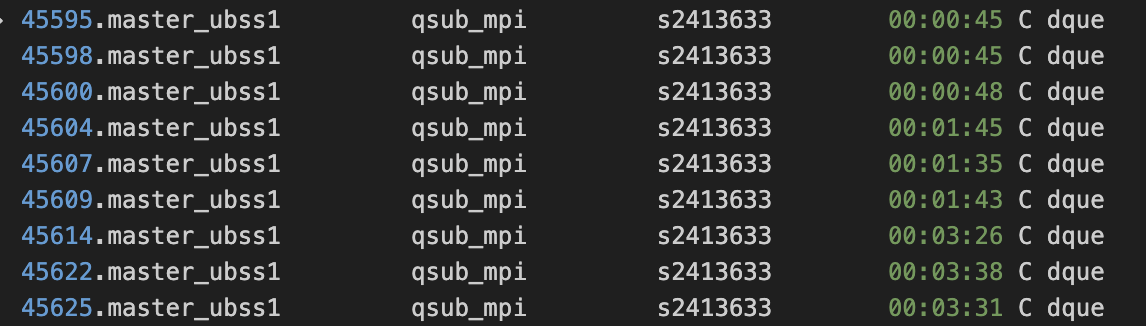
\includegraphics[width=0.9\textwidth]{1.png}
    \caption{7.1 重复实验原始时间结果}
    \label{fig:slot-time-np2-raw}
\end{figure}
\begin{figure}[H]
    \centering
    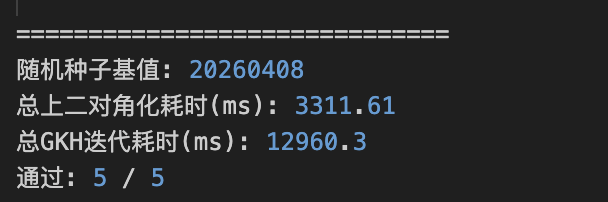
\includegraphics[width=0.4\textwidth]{2.png}
    \caption{np=2 测试实验中的一次截图}
    \label{fig:slot-time-np4-raw}
\end{figure}
\begin{figure}[H]
    \centering
    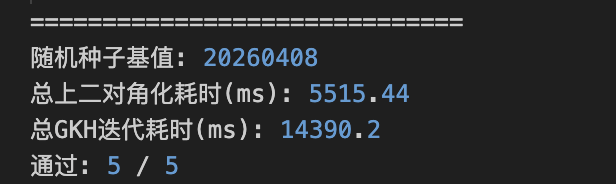
\includegraphics[width=0.4\textwidth]{3.png}
    \caption{np=4 测试实验中的一次截图}
    \label{fig:slot-time-np8-raw}
\end{figure}
\begin{figure}[H]
    \centering
    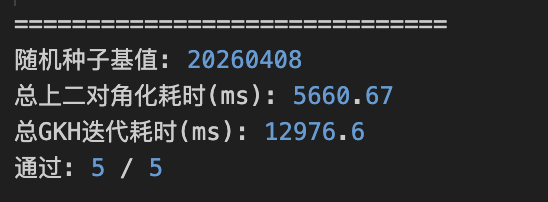
\includegraphics[width=0.4\textwidth]{4.png}
    \caption{np=8 测试实验中的一次截图}
    \label{fig:slot-time-server-shot}
\end{figure}

\subsection{为什么没加速：问题不只在通信，更在任务供给}

如果只看表~\ref{tab:gkh-time}，我们最多只能说“没加速”，因此我通过对代码的修改统计了一些时间参数：
\begin{enumerate}
    \item \texttt{time gkh iteration(ms)}：统计的是 GKH 这一段主计算过程在 root 端看到的关键路径时间，也就是这一部分真正花了多久。
    \item \texttt{MPI\_MAX wall}：统计的是一次并行执行里最慢那个进程的墙钟时间（大部分时间都是 rank=0 的主进程），更接近整轮任务实际完成所需要等待的时间。
    \item \texttt{comm subtotal}：统计的是收发任务、等待结果这些通信相关时间的总和，用来判断通信成本是不是已经比较重了。
    \item \texttt{task wait} 和 \texttt{result wait}：前者统计等新任务或等任务返回的时间，后者统计结果回收这一侧的等待时间，用来判断是不是有很多进程其实是在空等。
    \item \texttt{compute}：统计的是真正落在块计算上的时间，也就是实际做数值更新花掉的时间。
    \item \texttt{merge}：统计的是主进程把结果收回来之后，重新合并到全局矩阵并应用旋转的时间。
    \item \texttt{Time Use}：这是调度器记录的累计 CPU 使用时间，更像总资源的分配。
\end{enumerate}
\newpage
然后我们对 7.1 版本打印出来的 profiling 进行分析(这里展示的是三次重复的
平均值整理后的相同随机数种子\texttt{1000x1000} 样例)：

\begin{table}[h]
    \centering
    \scriptsize
    \caption{7.1 版本在 \texttt{1000x1000} 下的平均时间分解}
    \label{tab:profile-avg}
    \begin{tabular}{ccccccc}
        \toprule
        \texttt{np} & \texttt{MPI\_MAX wall}/ms & \texttt{comm subtotal}/ms &
        \texttt{task wait}/ms & \texttt{result wait}/ms & \texttt{compute}/ms & \texttt{merge}/ms \\
        \midrule
        2 & 12464.1 & 13153.5 & 5195.1  & 5723.8 & 4586.6 & 2719.8 \\
        4 & 13319.4 & 38210.0 & 30566.0 & 5552.6 & 4390.7 & 3333.2 \\
        8 & 12955.8 & 83857.1 & 76653.9 & 5593.2 & 4444.6 & 3074.1 \\
        \bottomrule
    \end{tabular}
\end{table}

这个表能看出两个很明显的现象。

第一，真正的 \texttt{compute} 时间几乎没有随着 \texttt{np} 增大而同步下降，基本都
还在 \(4.4\sim4.6\) 秒这个量级。这说明新增进程并没有把实打实的块计算量均匀分走。

第二，\texttt{task wait} 和整体 \texttt{comm subtotal} 却涨得非常快。\texttt{np=2}
时平均 \texttt{task wait} 只有 \(5.2\) 秒；到 \texttt{np=4} 时已经到了 \(30.6\) 秒；
\texttt{np=8} 时更是到了 \(76.7\) 秒。这个趋势非常说明问题：\textbf{进程确实开多了，
但是很多时候它们不是在算，而是在等。}

所以这里不能简单地说可能是拷贝、通信带来的时间增加，应该是：
\begin{enumerate}
    \item 主从框架和打包收发本身会带来额外开销；
    \item 但更核心的问题是，任务池并没有长期提供足够多的独立任务去喂满这些 worker；
    \item 在任务供给不足的前提下，进程数一加大，等待、收发、合并这些成本就会被放大出来。
\end{enumerate}

因此通过以上的分析，我们可以认为目前版本问题并不是单纯某一次
通信太慢，而是整个高层任务组织方式本身就很难把这些进程持续喂满。

\begin{figure}[H]
    \centering
    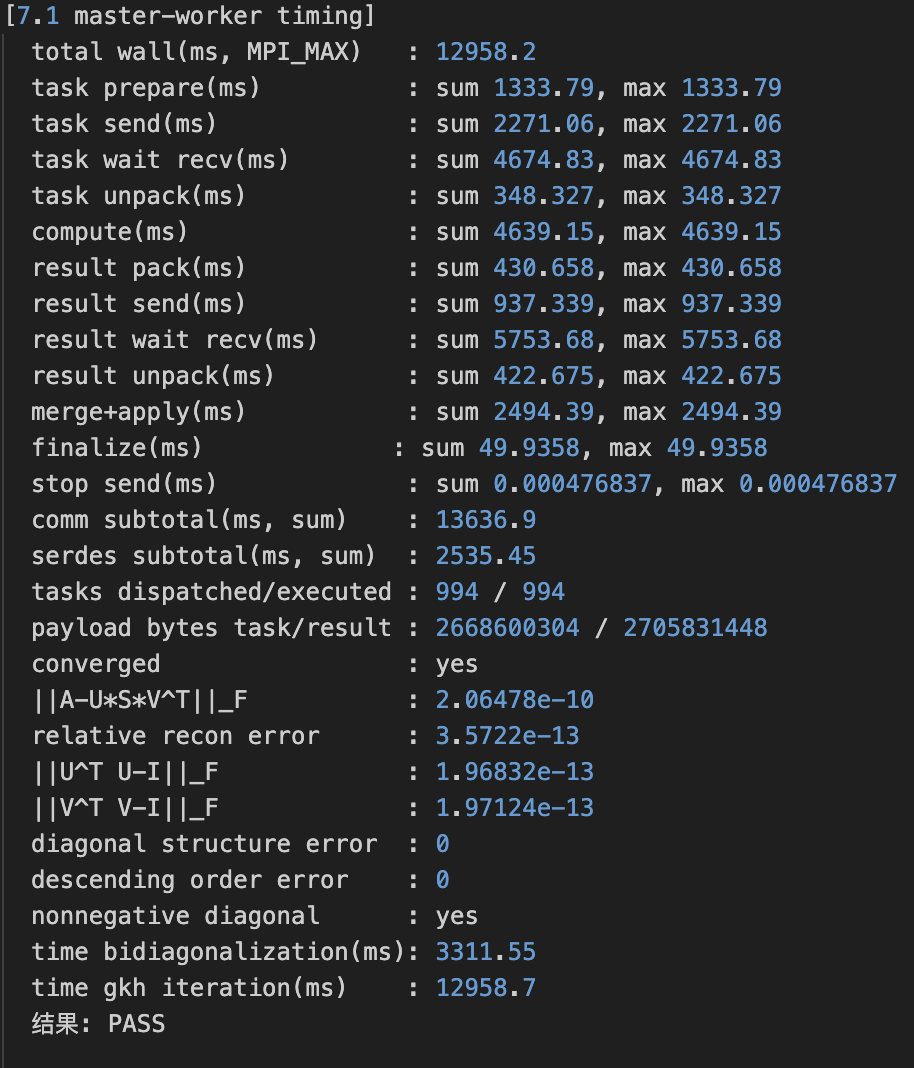
\includegraphics[width=0.4\textwidth]{5.png}
    \caption{np=2 测试实验中的一次 time}
    \label{fig:slot-profile-np2}
\end{figure}
\begin{figure}[H]
    \centering
    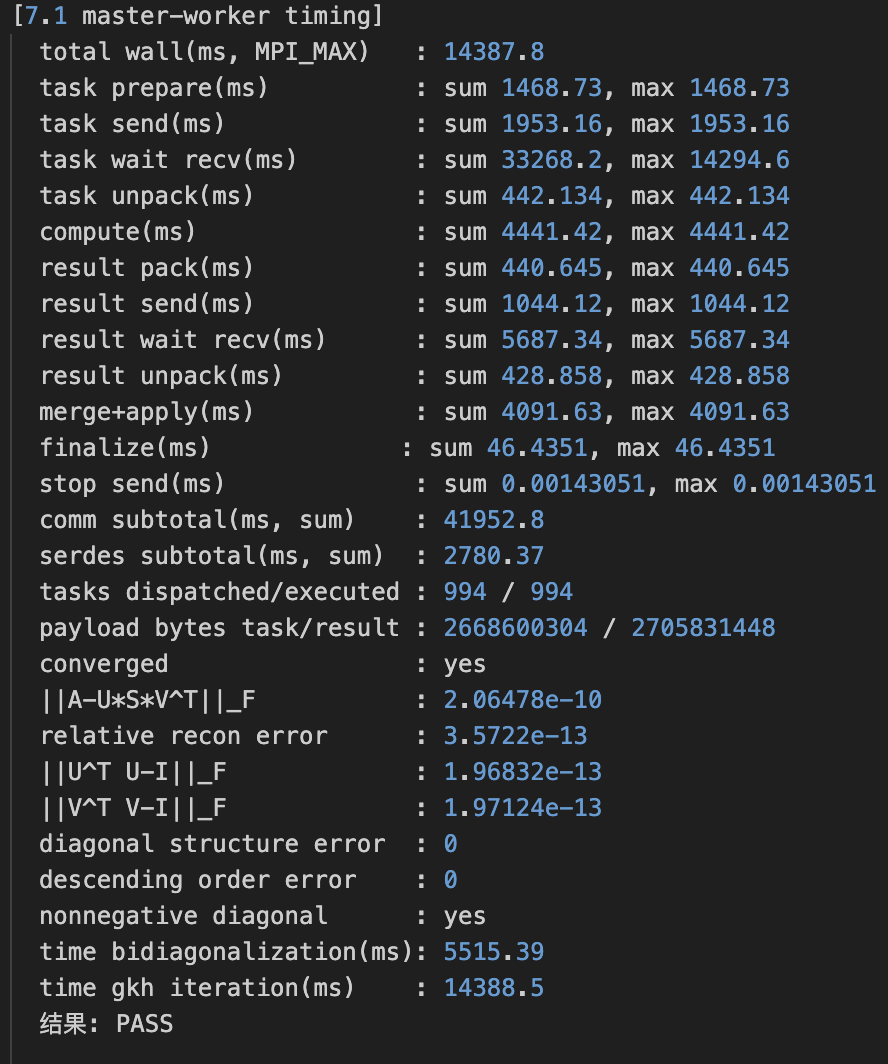
\includegraphics[width=0.4\textwidth]{6.png}
    \caption{np=4 测试实验中的一次time}
    \label{fig:slot-profile-np4}
\end{figure}
\begin{figure}[H]
    \centering
    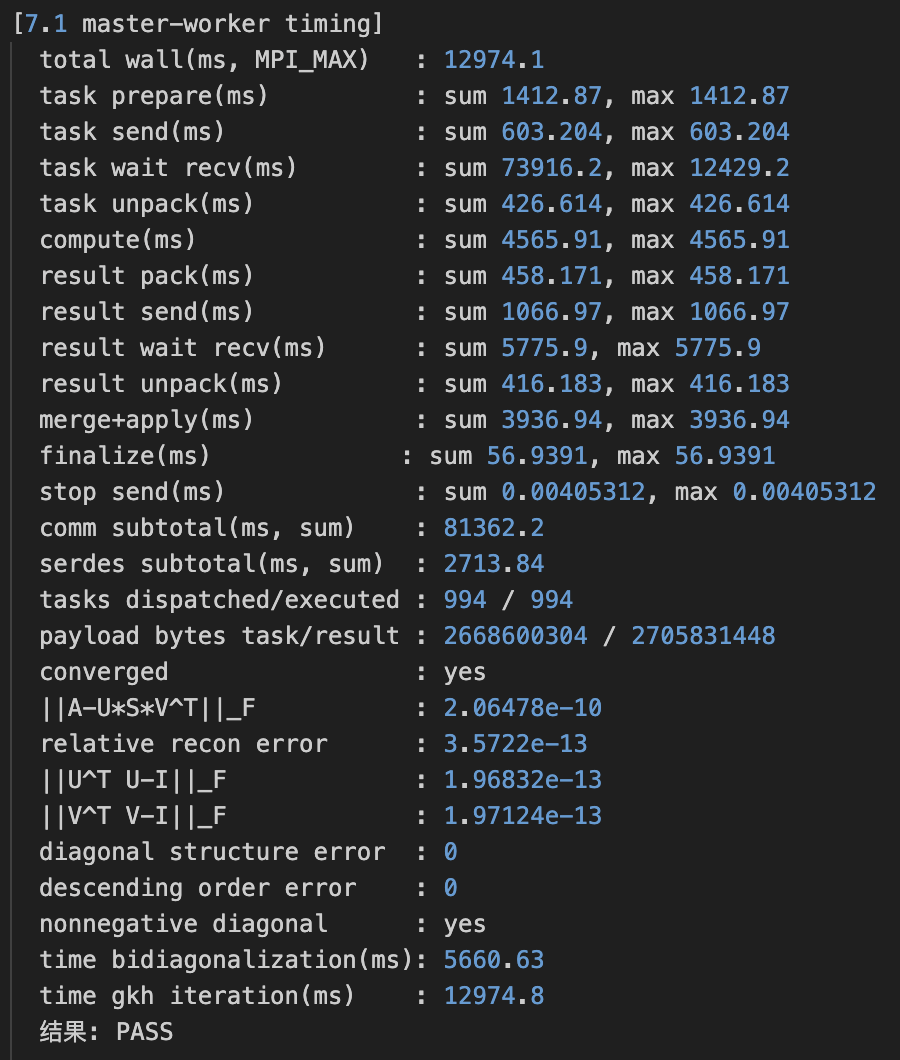
\includegraphics[width=0.4\textwidth]{7.png}
    \caption{np=8 测试实验中的一次time}
    \label{fig:slot-profile-np8}
\end{figure}

\subsection{和上次多线程实验的关系以及回答指导书中的7.3}

这一点其实正好能和上次的多线程实验接上。上次我已经感觉问题可能不只
是线程不够多，而是高层块任务本身就不太容易并行。到了这
次 MPI 实验，根据指导手册里的要求我换了多组随机种子，把每一轮的块信息打出来，想确认到底是不是
这里出了问题。打印代码如下：

\begin{lstlisting}
cleanup_bidiagonal(B, tol);
handle_diagonal_zeros_emit_ops(B, tol, u_ops, v_ops);

std::vector<Block> tmp_blocks = split_active_blocks(B, n, tol);
blocks.swap(tmp_blocks);

int non_singleton_count = 0;
for (size_t bi = 0; bi < blocks.size(); ++bi) {
    int len = blocks[bi].r - blocks[bi].l + 1;
    if (len > 1) ++non_singleton_count;
    std::cerr << len << ...;
}
\end{lstlisting}

它统计的是 \texttt{rank 0} 上全局矩阵 \(B\) 在当前轮
真正切出来的活动块。把 8 份日志汇总之后，
结果如表~\ref{tab:all-seeds} 所示。

\begin{table}[h]
    \centering
    \small
    \caption{8 个种子下非 \texttt{1x1} 活动块统计}
    \label{tab:all-seeds}
    \begin{tabular}{>{\raggedleft\arraybackslash}p{2.4cm}cccc}
        \toprule
        种子号 & 总轮数 & \texttt{non\_singleton=1} & \texttt{non\_singleton>1} & 占比 \\
        \midrule
        42       & 1491 & 1484 & 2  & 99.53\% \\
        2006     & 1489 & 1469 & 15 & 98.66\% \\
        20260409 & 1478 & 1459 & 14 & 98.71\% \\
        20260410 & 1491 & 1480 & 6  & 99.26\% \\
        20260411 & 1484 & 1469 & 10 & 98.99\% \\
        20260412 & 1486 & 1476 & 5  & 99.33\% \\
        20260607 & 1479 & 1464 & 10 & 98.99\% \\
        509896   & 1489 & 1478 & 6  & 99.26\% \\
        \bottomrule
    \end{tabular}
\end{table}
 因为日志太长，这里我也就只放一个局部截图，所有的 log 输出都已经在 log 子文件夹下，助教如果有需要可以直接查看：
\begin{figure}[H]
\centering
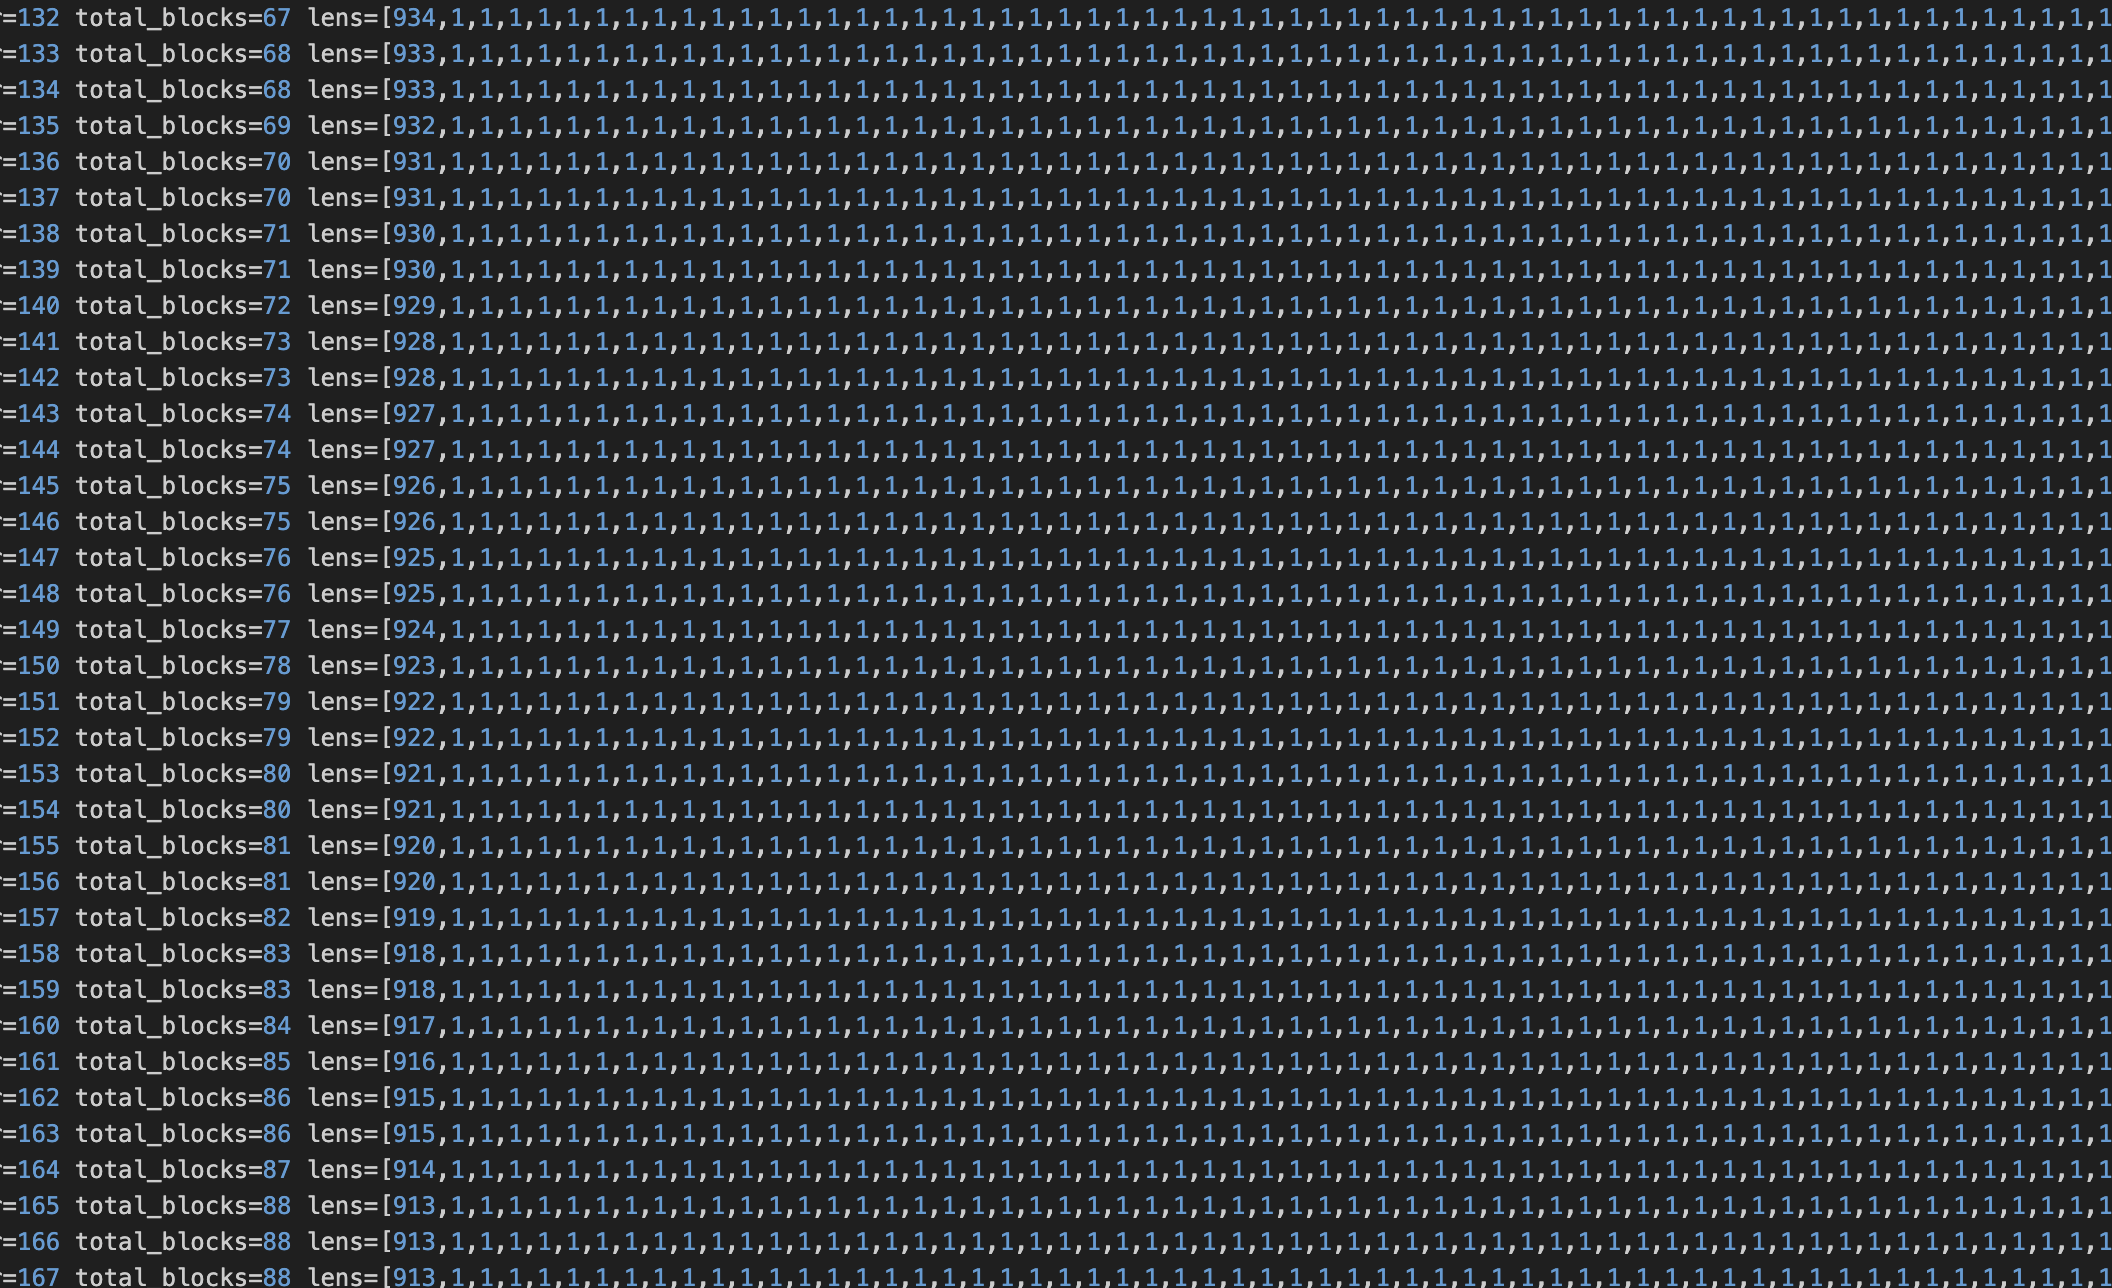
\includegraphics[width=0.9\textwidth]{8.png}
\caption{ 一次日志的局部截图}	
\end{figure}

我们回到这张表，通过分析我们可以看出：绝大多数轮次里，只有 1 个非 \texttt{1x1} 的活动块还在继
续推进，占比稳定在 \(98.66\%\sim99.53\%\) 之间。换句话说，\textbf{7.1.1 和 7.1.2
把并行框架搭出来以后，真正卡住它的，不是“没有任务池”，而是“任务池里大多数时候
根本没有足够多的非平凡块”。}

 因此我们就可以串起来我们的实验工作：
\begin{enumerate}
    \item 7.1.1 负责把主从和任务池搭起来；
    \item 7.1.2 负责把任务推进粒度改成按块推进；
    \item 7.3 则说明，这个任务池在绝大多数时候其实只能拿到 1 个真正可并行的非
          \texttt{1x1} 块。因此，新增进程没有办法长期拿到有效工作量，最后看到的就是资源用得更多，但时间并没有明显变快，这可以作为原因反过来解释 7.1 的工作结果差的原因。
\end{enumerate}

\section{两种 MPI 尝试}

在把 7.1.1 和 7.1.2 做完之后，我后面又继续尝试了两种不同的 MPI 写法。它们都还是围绕同一个
\texttt{gkh\_svd\_from\_bidiagonal} 展开，但在具体的进程职能划分上，思路并不一样。这里我把它们分别记成 \texttt{MPI1} 和 \texttt{MPI2}。

还需要说明的是我在多进程中对 main 进行了微小调整，只有 rank=0 的会进行打印输出，这是因为其他的进程都是 worker，拿到的都是不完整的数据，因此如果对这部分也进行校验打印出来的必定是fail。

\subsection*{MPI1：固定角色的三进程}

第一种尝试的思路比较直接，就是把三个进程的角色固定下来：
\begin{enumerate}
    \item \texttt{rank 0} 负责维护 \(B\)，并在 root 上推进块任务；
    \item \texttt{rank 1} 专门维护 \(U^T\)；
    \item \texttt{rank 2} 专门维护 \(V^T\)；
    \item 每次 root 处理完一个块之后，再把这一步产生的 \texttt{u\_ops} 和 \texttt{v\_ops} 分别发给另外两个进程。
\end{enumerate}

这一版我这里同样不把所有辅助函数都展开，而是只放一段最能说明思路的主干代码：

\begin{lstlisting}
if (rank == 0)
{
    Matrix Ut = transpose_copy(U);
    Matrix Vt = transpose_copy(V);
    send_matrix_to_rank(Ut, 1, TAG_UT_INIT, MPI_COMM_WORLD);
    send_matrix_to_rank(Vt, 2, TAG_VT_INIT, MPI_COMM_WORLD);

    while (!task_pool.empty() && task_budget < max_iter)
    {
        Matrix localB = extract_square_block(B, task.l, task.r);
        process_block_until_split(localB, tol, u_ops, v_ops, child_blocks);
        insert_square_block(B, localB, task.l);

        MPI_Send(&ctrl, 1, MPI_INT, 1, TAG_CTRL, MPI_COMM_WORLD);
        MPI_Send(&ctrl, 1, MPI_INT, 2, TAG_CTRL, MPI_COMM_WORLD);
        send_row_rotations_to_rank(u_ops, 1, TAG_U_TASK, MPI_COMM_WORLD);
        send_row_rotations_to_rank(v_ops, 2, TAG_V_TASK, MPI_COMM_WORLD);
    }
}
else if (rank == 1)
{
    Matrix Ut = recv_matrix_from_rank(m, m, 0, TAG_UT_INIT, MPI_COMM_WORLD);
    apply_row_rotations_local(Ut, u_ops);
}
else if (rank == 2)
{
    Matrix Vt = recv_matrix_from_rank(n, n, 0, TAG_VT_INIT, MPI_COMM_WORLD);
    apply_row_rotations_local(Vt, v_ops);
}
\end{lstlisting}

这段代码就是先把 \(U^T\) 和 \(V^T\) 分别交给两个固定进程保管，然后 root 每处理完一个块，就把这一轮产生的旋转操作分别发出去，让另外两个进程各自更新自己的矩阵。

这一版的优点是角色很清楚，但缺点也很明显，就是这种方式把并行结构固定死在了\texttt{np=3} 上，而且 root 仍然承担了主要的块推进工作，而不是一个可以自然扩展到更多进程的通用版本。

\begin{table}[H]
    \centering
    \scriptsize
    \caption{MPI1 在 \texttt{1000x1000} 下的 profiling 均值（5 次重复）}
    \label{tab:mpi1-results-slot}
    \begin{tabular}{ccccccccc}
        \toprule
        进程数 & 通过次数 & GKH均值/ms & 关键路径Wall/ms & Root处理/ms & Root抽取回填/ms & 通信累计/ms & 更新累计/ms & Time Use/s \\
        \midrule
        3 & 5 / 5 & 5851.45 & 6051.10 & 4455.22 & 927.35 & 9904.09 & 1842.37 & 48.4 \\
        \bottomrule
    \end{tabular}
\end{table}

这里我统计的都是大矩阵 \texttt{1000x1000} 这一档，因为真正能拉开差距的主要就是这一组。从这张表里可以看到，
\texttt{MPI1} 这一版是能稳定跑通的，5 次重复都是 \texttt{5/5 PASS}。它的 rank=0主进程GKH 时间均值是
\(5851.45\text{ ms}\)，我们相比于 7.1 的版本进行了加速。表里的“关键路径Wall”统计的是
\texttt{MPI\_MAX wall}，也就是整轮执行真正决定总耗时的那条关键路径；而“通信累计”和“更新累计”统计的是把
所有进程上的对应时间全部加起来之后的结果，所以它们不能直接和 \texttt{GKH} 或 \texttt{Wall} 去逐项相加。
因此我们可以看到，rank=0 自己处理块的时间均值已经到了 \(4455.22\text{ ms}\)，
rank=0 抽取和回填块又花了 \(927.35\text{ ms}\)，说明主要工作还是压在 rank=0 上；与此同时，三进程合起来累计在通信上又花了
\(9904.09\text{ ms}\)，说明这套固定角色方案在全体进程上的通信成本也并不低。也就是说，这一版并行结构依旧是还是很偏向 rank=0 的，另外两个进程是在辅助计算。

\begin{figure}[H]
    \centering
    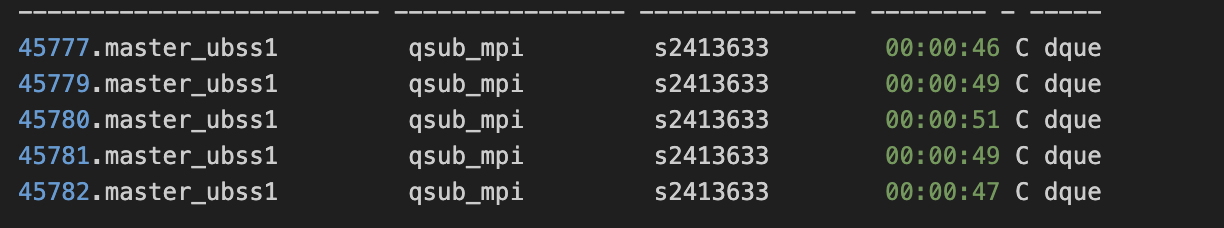
\includegraphics[width=0.9\textwidth]{9.png}
    \caption{固定角色的结果}
    \label{fig:slot-mpi1-result}
\end{figure}
\begin{figure}[H]
    \centering
    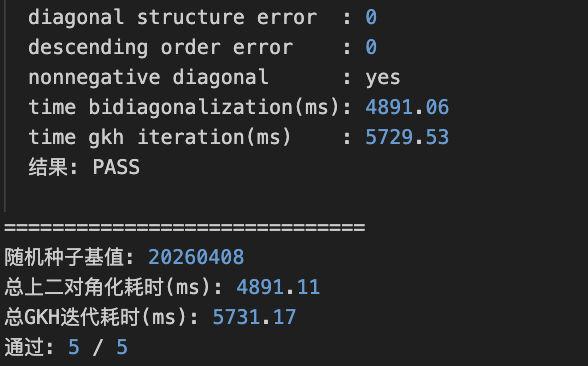
\includegraphics[width=0.5\textwidth]{10.png}
    \caption{固定角色的结果二（局部截图）}
    \label{固定角色的结果二}
\end{figure}

\subsubsection*{MPI2：列块分发加广播同步的通用方案}

这一版我当时想解决的核心问题是：
既然第一种写法把进程角色固定死了，那能不能改成一个更一般的方案，让所有进程都真正参与到
\(U^T\) 和 \(V^T\) 的更新里来。

这里还有一个思路上的取舍需要先说清楚。按直觉看，最想并行的当然还是 \(B\) 本身，因为真正的
GKH 推进主要都发生在 \(B\) 上。但问题在于，\(B\) 这一侧的块推进有很强的连续性：当前这一轮怎么切块、
下一步追到哪里、块什么时候重新分裂，这些都强依赖前一步刚刚算出来的结果，所以它并不适合像普通数据并行那样，
直接把 \(B\) 很自然地切给多个进程同时独立推进。正因为这一层不好直接做进程化，我这里才换了一个角度，
去尝试把 \(U^T\) 和 \(V^T\) 的更新拆给多个进程，让 主进程 继续维护 \(B\)，而其他进程去并行承担旋转应用这一部分。

但这样做也有一个很自然的预期：\(U^T\) 和 \(V^T\) 的更新虽然可以拆开，但它们本身并不是这整个流程里最重的那一部分。
如果为了让所有进程都参与进来，反而要额外付出列块分发、广播旋转、最终 gather 回收这些成本，那么最后很可能出现的情况就是：
通信和拷贝的代价比真正省下来的计算还大。所以从思路上说，\texttt{MPI2} 这版虽然更通用，但有可能因为同步和通信更重，最后反而更慢。

所以这一次的思路变成了：
\begin{enumerate}
    \item 先把 \(U^T\) 和 \(V^T\) 按列块切开，分发给所有进程；
    \item root 还是负责维护 \(B\) 并推进块任务；
    \item 每处理完一个块，root 把这一轮生成的旋转操作广播给所有进程；
    \item 每个进程只在自己手里的局部列块上应用这些旋转；
    \item 最后再把各自的列块 gather 回 root，拼成完整的 \(U^T\) 和 \(V^T\)。
\end{enumerate}

主干代码如下：

\begin{lstlisting}
if (rank == 0)
{
    Ut_local = scatter_col_blocks_from_root(Ut_full, m, m, 0, MPI_COMM_WORLD);
    Vt_local = scatter_col_blocks_from_root(Vt_full, n, n, 0, MPI_COMM_WORLD);
}
else
{
    Ut_local = scatter_col_blocks_from_root(dummy_u, m, m, 0, MPI_COMM_WORLD);
    Vt_local = scatter_col_blocks_from_root(dummy_v, n, n, 0, MPI_COMM_WORLD);
}

while (true)
{
    if (rank == 0)
    {
        Matrix localB = extract_square_block(B, task.l, task.r);
        process_block_until_split(localB, tol, u_ops, v_ops, child_blocks);
        insert_square_block(B, localB, task.l);
    }

    MPI_Bcast(&control, 1, MPI_INT, 0, MPI_COMM_WORLD);
    bcast_row_rotations(u_ops, 0, MPI_COMM_WORLD);
    bcast_row_rotations(v_ops, 0, MPI_COMM_WORLD);
    apply_row_rotations_local(Ut_local, u_ops);
    apply_row_rotations_local(Vt_local, v_ops);
}

Matrix Ut_gathered = gather_col_blocks_to_root(Ut_local, m, m, 0, MPI_COMM_WORLD);
Matrix Vt_gathered = gather_col_blocks_to_root(Vt_local, n, n, 0, MPI_COMM_WORLD);
\end{lstlisting}

这段代码的意思是：先把完整矩阵拆成每个进程各管一块，然后由 root 统一广播每一步产生的旋转操作，所有进程再同步更新自己手里的局部列块。

这部分的时间统计如下：

\begin{table}[H]
    \centering
    \scriptsize
    \caption{MPI2 在 \texttt{1000x1000} 下的 profiling 均值（分别三次平均值）}
    \label{tab:mpi2-results-slot}
    \begin{tabular}{ccccccccc}
        \toprule
        进程数 & 通过次数 & GKH均值/ms & 关键路径Wall/ms & 主进程处理/ms & 主进程抽取回填/ms & 通信累计/ms & 更新累计/ms & Time Use/s \\
        \midrule
        2 & 3 / 3 & 7896.71 & 7896.19 & 5082.59 & 1007.04 & 6746.12  & 2210.70 & 35.3 \\
        4 & 3 / 3 & 7694.35 & 7931.81 & 5218.42 & 1056.86 & 20983.20 & 2235.08 & 80.3 \\
        8 & 3 / 3 & 7166.82 & 8005.29 & 4903.31 & 983.93  & 49006.93 & 2162.94 & 177.3 \\
        \bottomrule
    \end{tabular}
\end{table}

首先这一版在 \texttt{np=2,4,8} 下都能稳定跑通，三次重复也都是 \texttt{5/5 PASS}。
再看时间，\texttt{time gkh iteration(ms)} 的均值确实有一点下降，
从 \texttt{np=2} 的 \(7896.71\text{ ms}\) 降到了 \texttt{np=8} 的 \(7166.82\text{ ms}\)。但如果把
\texttt{MPI\_MAX wall} 和 \texttt{Time Use} 放在一起看，问题就出来了：墙钟时间并没有跟着明显下降，
基本一直在 \(7.9\sim8.0\text{ s}\) 这一带，而 \texttt{Time Use} 却从 \(35.3\text{ s}\) 一路涨到了
\(177.3\text{ s}\)。

更关键的是通信项。\texttt{comm subtotal} 从 \texttt{np=2} 的 \(6746.12\text{ ms}\) 直接涨到
\texttt{np=8} 的 \(49006.93\text{ ms}\)，增长非常明显。因此我们可以分析出随着进程数增加，
有效计算没有随之变多，广播、同步和回收这些成本也符合我们预期上升的比较明显。

所以 \texttt{MPI2} 这一版虽然结构更通用，但是在当前 SVD 这类任务下，进程一加多，通信负担会被非常快地放大出来。

\begin{figure}[H]
    \centering
    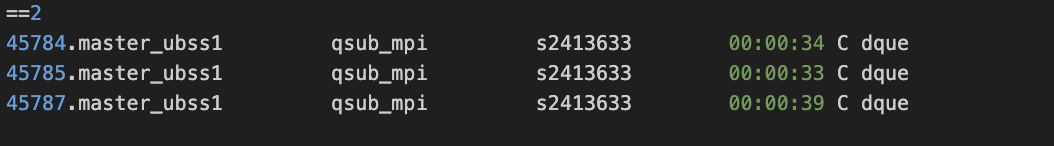
\includegraphics[width=0.9\textwidth]{11.png}
    \caption{MPI2：np=2的结果}
    \label{fig:slot-mpi2-np2-full}
\end{figure}
\begin{figure}[H]
    \centering
    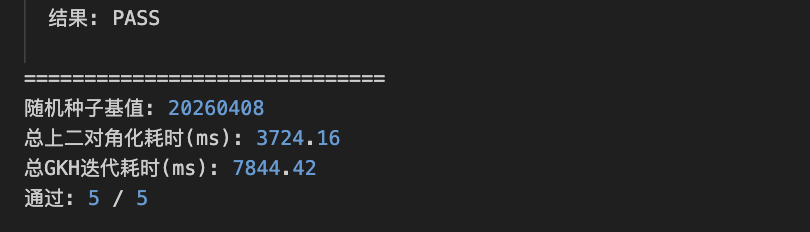
\includegraphics[width=0.5\textwidth]{12.png}
    \caption{MPI2：np=2的结果二（局部截图）}
\end{figure}

\begin{figure}[H]
    \centering
    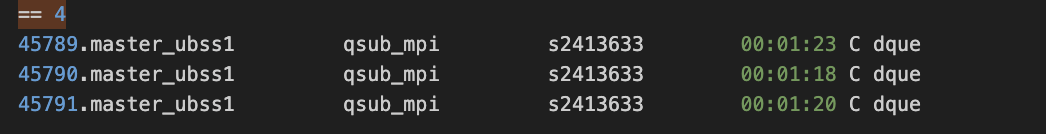
\includegraphics[width=0.9\textwidth]{13.png}
    \caption{MPI2：np=4的结果}
    \label{fig:slot-mpi2-np4-full}
\end{figure}
\begin{figure}[H]
    \centering
    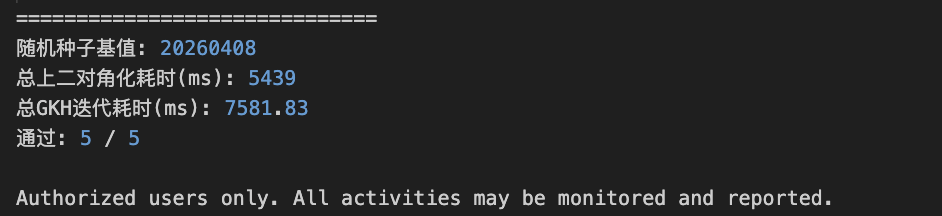
\includegraphics[width=0.5\textwidth]{14.png}
    \caption{MPI2：np=4的结果二（局部截图）}
\end{figure}

\begin{figure}[H]
    \centering
    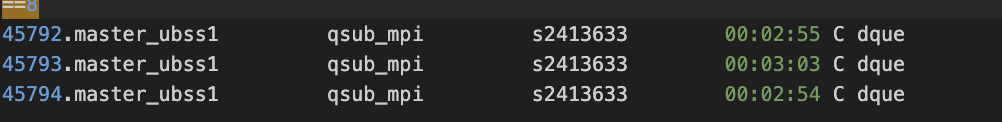
\includegraphics[width=0.9\textwidth]{15.png}
    \caption{MPI2：np=8的结果}
    \label{fig:slot-mpi2-np8-full}
\end{figure}
\begin{figure}[H]
    \centering
    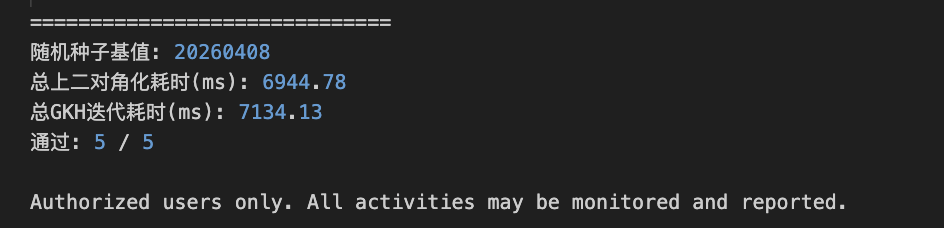
\includegraphics[width=0.5\textwidth]{16.png}
    \caption{MPI2：np=8的结果二（局部截图）}
\end{figure}
\section{总结}
这次实验我们围绕 SVD 的 GKH 迭代，连续尝试了几条不同层次的多进程并行化。最开始做的是把原来按外层迭代整体推进的写法，改成按非 1x1 活动块推进，并在这个基础上搭出主从和任务池框架。之后，我们又继续尝试了两种 MPI 写法：一种是固定角色的三进程方案，由主进程维护 B，另外两个进程分别维护$ U^T $和 $V^T$；另一种是更通用的列块分发
  加广播同步方案，让更多进程一起参与 $ U^T $和 $V^T$ 的更新。

  从结果上看，首先，7.1 这一层说明主从和任务池是能搭起来的，程序也能稳定跑通，但提高进程数以后并没有得到明显加速。接着，再结合日志统计可以看到，绝大多数时候实际上只有一个非 1x1 的活动块在继续推进，这就意味着高层任务池里长期没有足够多的独立任务去喂满这些进程； 之后MPI 中尝试固定三角色的方案结果相对更快；更通用的广播同步方案虽然能自然扩展到更多进程，但随着进程数增加，通信、同步和数据分发的开销涨得非常快。

  如果说这次实验最大的收获，是我对profiling 有了更深层的理解，因为很多现象只看总时间是看不出来的，必须把关键路径、通信累计、等待、局部更新这些细节子量拆开，才能知道问题到底卡在哪。

\newpage
\appendix
\section{AI 使用说明附录}
这一部分主要记录我在实验分析阶段，如何借助 AI 一起把 profiling 的口径一步一步定下来。

\subsection{1. 一开始关心的问题}

我在后面开始写 profiling 的时候，是到底应该统计哪些时间。因为这次实验里有主进程、有子进程、有点对点通信、有广播同步，还有一些看起来很像时间、但含义其实不一样的量。如果这里口径没定好，后面所有分析都会很乱。

当时我主要围绕下面几个问题和 AI 讨论：
\begin{enumerate}
    \item 如果想说明程序真正有没有变快，关键路径(rank=0)应该怎么统计。
    \item MPI 里有哪些现成 API 可以用来做时间统计。
    \item 哪些量适合拿来说明“用户实际等了多久”，哪些量适合拿来说明“总资源消耗有多大”。
\end{enumerate}

\subsection{2. 我和 AI 的问答记录}

\textbf{我问：如果想说明程序真正有没有变快，关键路径（rank=0）应该怎么统计？}

\textbf{AI答：} 如果只是想回答“这个程序最后到底有没有变快”，那最应该优先看的不是所有进程加起来花了多少时间，而是关键路径上到底花了多少时间。因为对用户来说，真正关心的是这一轮程序什么时候结束，而不是后台一共累计消耗了多少时间。

具体到这次实验里，可以先看 \texttt{time gkh iteration(ms)}，因为它直接对应的是这一段 GKH 迭代主流程在 root 端看到的运行时间；如果想再严格一点，就看 \texttt{MPI\_MAX wall}，也就是所有进程里最慢那个进程的墙钟时间。这个量更接近“整轮任务真正完成时，所有人一共等了多久”。

因此最后在报告里，我就把关键路径时间单独拿出来看，而不是一上来把所有统计量混在一起。

\textbf{我问：MPI 里有哪些现成 API 可以用来做时间统计？}

\textbf{AI答：} 这次最直接、最好用的其实就是 \texttt{MPI\_Wtime()}。它适合做 MPI 程序内部的分段计时，比如：
\begin{enumerate}
    \item 在 root 开始处理一个块之前记一次时间；
    \item 在处理结束之后再记一次时间；
    \item 两次相减，就能得到这一段 \texttt{root process block} 的时间。
\end{enumerate}

同样的方法也可以拿去统计：
\begin{enumerate}
    \item 收发控制消息的时间；
    \item 广播旋转操作的时间；
    \item 本地应用旋转的时间；
    \item 最后 gather 或 collect 的时间。
\end{enumerate}

也就是说，这次不是用一个特别重的外部 profiler 去一次性看全局，而是优先在代码里自己埋时间点，把流程拆开来记。这样做的好处是每个时间量的含义都很明确，后面写报告时也比较容易解释。

\textbf{我问：哪些量适合拿来说明“用户实际等了多久”，哪些量适合拿来说明“总资源消耗有多大”？}

\textbf{AI答：} 这里最容易混掉，所以后来我和 AI 反复确认过，最后把这些量分成了两层。

第一层是“用户实际等了多久”。这一层主要看：
\begin{enumerate}
    \item \texttt{time gkh iteration(ms)}
    \item \texttt{MPI\_MAX wall}
\end{enumerate}
因为这两个量都更接近关键路径，也就是程序真正结束前用户需要等待的时间。

第二层是“总资源消耗有多大”。这一层主要看：
\begin{enumerate}
    \item \texttt{comm subtotal}
    \item \texttt{local update}
    \item 调度器里的 \texttt{Time Use}
\end{enumerate}

其中 \texttt{comm subtotal} 和 \texttt{local update} 是把多个进程上的对应时间累计起来之后得到的，所以它们可以比关键路径更大；而 \texttt{Time Use} 更像整个作业一共吃掉了多少 CPU 资源。也正是因为这几个量不是一个层次，所以后面我才把表头改成了“关键路径Wall”“通信累计”“更新累计”这种说法，避免把它们误看成能直接相加的同类时间。

\subsection{3. 最后形成的分析口径}

基于上面这些问答，最后我在报告里真正采用的 profiling 口径就是：
\begin{enumerate}
    \item 用 \texttt{time gkh iteration(ms)} 和 \texttt{MPI\_MAX wall} 看关键路径；
    \item 用 \texttt{root process block} 和 \texttt{root extract+insert} 看主进程本地负担；
    \item 用 \texttt{comm subtotal} 看总体通信负担；
    \item 用 \texttt{local update} 看各进程本地更新量；
    \item 用调度器的 \texttt{Time Use} 看整次作业的总资源消耗。
\end{enumerate}

这样做的好处是，如果后面程序没有加速，我就不会只得到一个“没有变快”的结论，而是还能继续往下分辨：它到底是卡在 root、卡在通信同步，还是卡在高层任务本身就喂不满这些进程。
\end{document}
